% !TEX root       = ./type_name.tex
% !TEX program    = pdflatex
% !TEX encoding   = utf-8
% !TEX spellcheck = de_DE_frami
% Please add the following required packages to your document preamble:
%\usepackage{booktabs}
%\usepackage{graphicx}
%\usepackage[table,xcdraw]{xcolor}
% If you use beamer only pass "xcolor=table" option, i.e. \documentclass[xcolor=table]{beamer}
%=======================================================================

\chapter{Control and Authentication Mechanism}\label{ch:control_and_authentication}
\sffamily{}

In this chapter, the softwares and protocols used for providing authentication and for controlling the access point is discussed. A brief introduction to OpenWrt and the different protocols such as OpenFlow, RADIUS is described in the flowing topics.
\section{OpenWrt \cite{WhatIsOpenWrt}} \label{OpenWrt}

OpenWrt is a Linux distribution that works like any other Linux distro designed for embedded devices. OpenWrt offers bult-in package manager that allows to install packages from its repository or manually build your own firmware file using your custom-built package. The packages range anything from an SSH server, VPN, traffic-shaping, enterprise wireless solutions, BitTorrent client, or even as a hotspot manager.

OpenWrt is designed for power users that wants customizability to the stock firmware provided by the manufacturer. There are many custom firmware’s such as DD-WRT available for most popular routers, for this thesis, OpenWrt is chosen because of its flexibility and more stable than most custom firmware’s or sometimes even the stock firmware.

OpenWrt has many features that can be mentioned but out of scope for this thesis, a run-down version of the most relevant features are listed below that are related to this thesis.

\begin{itemize}
	\item \textbf{SSH server for terminal access:} Provides SSH server, which allows to connect directly to the routers terminal via SSH and when the router is configured to the internet, allows to remotely configure the router. 
	\item \textbf{Capture and Analyse network Traffic:} Tcpdump tool is included in the build to analyze the packets that are traversing thru the router. The tool can also be used to create packet logs that can be open in packet analyzer tools such as Wireshark.
	\item \textbf{GUI Interface:} OpenWrt also includes a GUI interface for managing most of the router’s configuration, the built in one is named as LuCi.
	\item \textbf{OpenvSwitch:} The virtual switch is also available as a package on OpenWrt repository that is used in this thesis to be installed in the router for creating a virtual switch within the router that can also work along with the physical switched present.
	\item \textbf{Wireless Utilities:} OpenWrt provides many different packages for managing wireless sockets in the router, for this thesis, Hostapd package is chosen because of its fully featured support for a wide range of authentication mechanisms such as IEEE 802.1x/WPA/EAP/RADIUS with EAP protocols. It can be configured in the file located at /etc/hostapd.conf in the routers folder.
	\item \textbf{Freeradius:} The open source RADIUS server is also available as a package for the OpenWrt build but is not used in the firmware for this thesis because of memory unavailability of the TP Link WR-4300 router.
	\item \textbf{MySQL:} The is a fully featured MySql server also available as the packages that can be installed on the router but again could not be used in this thesis due to memory restrictions of the router.
	
\end{itemize}
The following figures below shows the SSH interface of OpenWrt terminal and the LuCi web interface.
\begin{figure}[H]
	\centering
	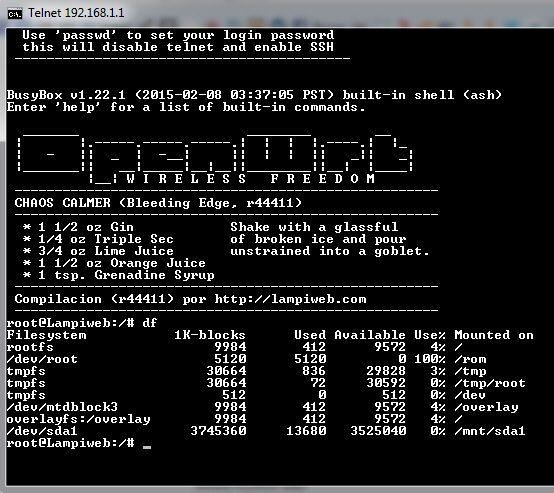
\includegraphics[width=1.0\linewidth]{openwrt4-terminal}
	\caption{OpenWrt Terminal View \cite{openwrt_terminal_img}} \label{fig:OpenWrt_terminal}
	\vspace{-10pt}
\end{figure}

\begin{figure}[H]
	\centering
	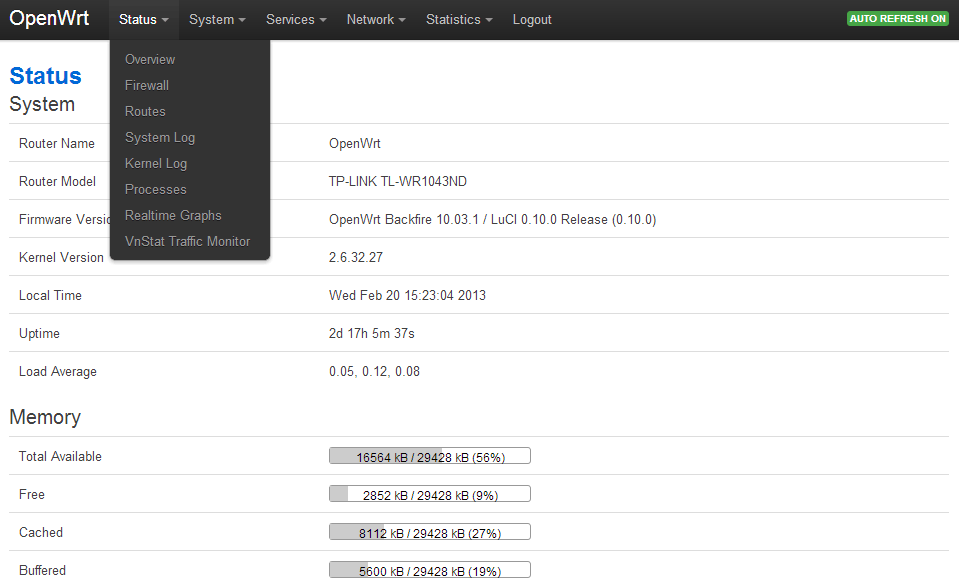
\includegraphics[width=1.0\linewidth]{bootstrap-luci-theme}
	\caption{OpenWrt GUI Interface \cite{openwrt_luci_img}} \label{fig:OpenWrt_gui}
	\vspace{-10pt}
\end{figure}
\section{Protocols} \label{protocols}
For this thesis, protocols such as OpenFlow, RADIUS and 802.1x security are used extensively and are discussed in detail below, explaining their use cases and features.
\subsection{OpenFlow \cite{WhatIsOpenFlow}} \label{OpenFlow}

It is a standard communication interface defined between the control and forwarding layers of the SDN architecture, allowing direct access for manipulating the forwarding plane of the network devices such as switches and routers, both physical and virtual (hypervisor based).

OpenFlow, along with SDN technologies have helped IT to manage and address the high-bandwidth, and dynamic nature of today’s applications. It also has helped adapt the network to ever-changing business needs, and significantly reduce the complexity in maintenance and operations.

Some of the best features of OpenFlow is explained in the following figure.

\begin{figure}[H]
	\centering
	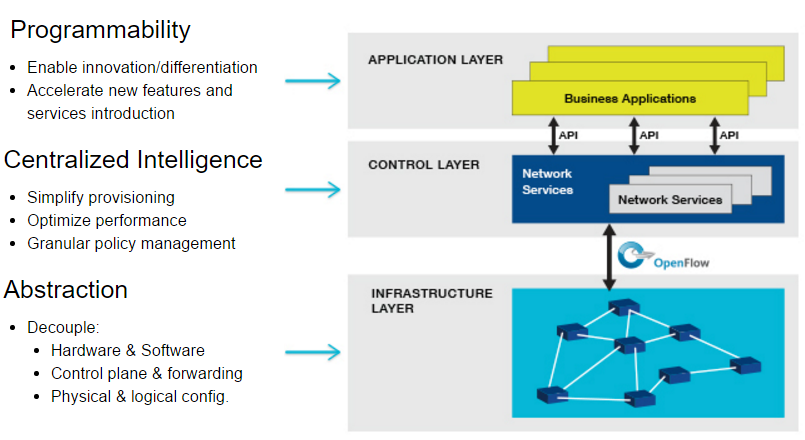
\includegraphics[width=1.0\linewidth]{of-features}
	\caption{OpenFlow features \cite{openflow_features}} \label{fig:OF_features}
	\vspace{-10pt}
\end{figure}

\subsubsection{How does OpenFlow Work? \cite{OpenFlow_functionality}} \label{OpenFlow_Functionality}
In a traditional switch or a router, the packet forwarding and high level routing decisions occur on the same device. In an OpenFlow switch, the routing and forwarding functions are separated. The data path portion is still on the switch and the routing decisions are handled by a separate controller, typically it’s a standard server. The OpenFlow switch and controller communicate using the OpenFlow protocol, which defines messages such as packet-in, packet-out modify-forwarding path and get stats.
\subsubsection{OpenFlow Specification \cite{Openflow_protocol_spec}} \label{OpenFlow_Protocol_spec}
The protocol can be split into 4 components namely: message layer, state machine, system interface and configuration. 
\begin{figure}[H]
	\centering
	\includegraphics[width=1.0\linewidth]{of-protocol}
	\caption{OpenFlow Protocol \cite{of_protocol_spec_img}} \label{fig:Of_proto}
	\vspace{-10pt}
\end{figure}

\begin{itemize}
	\item \textbf{Message Layer:} 
	\\ It is the core of the protocol stack. It also supports the ability to construct, copy, compare, manipulate and print the messages. The message layer defines the valid structure and semantics for all messages.   
	\item \textbf{State Machine:}
	\\ It defines the core level behaviour of the protocol. It is typically used to describe the actions such as: flow control, negotiations, delivery, capability discovery etc.
	\item \textbf{System Interface:}
	\\ It typically defines how the protocol interacts with the other protocols in the outside world. The system interface identifies the necessary and optional interfaces along with its intended use such as TLS and TCP as transport channels.
	\item \textbf{Configuration:}
	\\ Almost every protocol has its own configuration or initial values. It can cover anything from buffer size, reply intervals to X.509 certificates.
	\item \textbf{Data Model:}
	\\ Each switch maintains the attributes of each OpenFlow abstration in a relational data model.  The attributes either describe its configuration state, or some set of current statistics or the abstraction capability. 

\end{itemize}

\subsubsection{OpenFlow Switch \cite{Opnflow_switch}} \label{OpenFlow_Switch}

 An OpenFlow switch is made up of two components namely the switch agent and the data plane. The switch agent takes care of the communication between two or more controllers and also with the data plane using the requisite internal protocol. The switch agent translates the commands into low-level instructions to send to the data plane and the data plane notifications to the OpenFlow messages that are forwarded to the controller. The data plane takes care of the packet manipulation and forwarding and sometimes sends packets to the switch agent for further handling based on its configuration.
 
\begin{figure}[H]
 	\centering
 	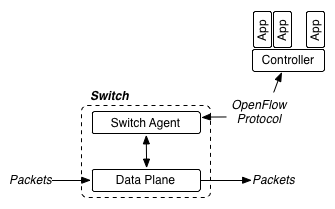
\includegraphics[width=1.0\linewidth]{of-switch-anatomy}
 	\caption{OpenFlow Switch Anatomy \cite{Of_Switch_img}} \label{fig:Of_switch_anatomy}
 	\vspace{-10pt}
\end{figure}
 
\subsubsection{OpenFlow Switch Agent \cite{Opnflow_switch}} \label{Of_switch_agent}
 The following figure shows how the switch agent works, its components are explained the table following the figure.
 
\begin{figure}[H]
 	\centering
 	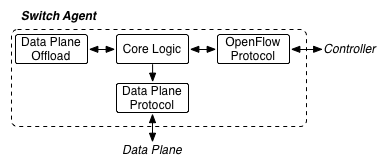
\includegraphics[width=1.0\linewidth]{of-switch-agent-anatomy}
 	\caption{OpenFlow Switch Agent \cite{Of_Switch_agent_img}} \label{fig:Of_switch_agent}
 	\vspace{-10pt}
\end{figure}

\begin{itemize}
	\item \textbf{OpenFlow protocol:} This instance is on the switch side
	\item \textbf{Core Logic:} Switch management, command execution to the data plane and manage the data plane offload etc.
	\item \textbf{Data Plane Offload:} Some functionality present in the OpenFlow will be offloaded by the control plane which is not provided in the existing data plane implementation.
	\item \textbf{Data Plane protocol:} This protocol is internal which is mostly used for configuring the data plane state.
	
\end{itemize}

\subsubsection{Data Plane \cite{Opnflow_switch}} \label{of_data_plane}

The data plane consists of the ports, flow tables, flows, classifiers and actions. Packets traverse through the system on ports. When each packet arrives, it is matched with the flows in the flow table using classifiers. The flows contain the set of actions that are applied to each packet that matches.

\begin{figure}[H]
	\centering
	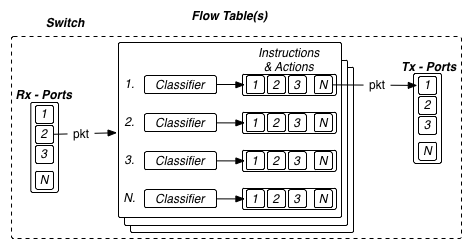
\includegraphics[width=1.0\linewidth]{Of-data-plane-flow}
	\caption{OpenFlow Data Plane Schematic \cite{Of_data_plane_flow_img}} \label{fig:Of_data_plane_img}
	\vspace{-10pt}
\end{figure}

\subsubsection{Data Plane - Packet Lifecycle \cite{Opnflow_switch}} \label{of_data_plane_lifecycle}

Each packet is processed in the following sequence as explained in the table below.
\begin{figure}[H]
	\centering
	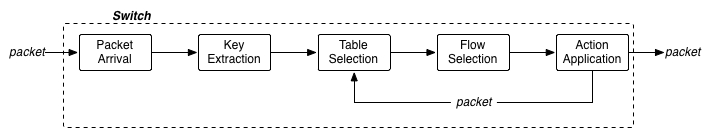
\includegraphics[width=1.0\linewidth]{Of-packet-lifecycle}
	\caption {Packet Lifecycle \cite{Of_packet_lifecycle}}
	\label{fig:of_packet_lifecycle}
	\vspace{-10pt}
\end{figure}

\begin{itemize}
	\item \textbf{Step 1: Packet Arrival}
	\\ Packets arrive in either a physical or virtual port, it is necessary to make note of the arrival port for source-based processing later.
	\item \textbf{Step 2: Key Extraction}
	\\ When each packet arrive on the port, a small meta data is built called the key. This key contains information about the packet such as header values, buffered packet, arrival port, arrival time etc. 

	\item \textbf{Step 3: Table Selection}
	\\ When a packet goes through the pipeline, the packet is matched with the first table by default and if multiple tables exist then subsequent tables will be selected through hit or miss actions.
	\item \textbf{Step 4: Flow Selection}
	\\ The Key extracted in the initial step is used for selecting the flow from the table. The first flow where the classifier subsumes the key become the selected flow.
	\item \textbf{Step 5: Application Selection}
	\\ Each flow contains a set of actions, which is applied to the packet when a flow is matched. The actions can modify the state of the packet or change how the packet is treated. 
	
\end{itemize}

\subsection{RADIUS \cite{RADIUS_RFC2865}} \label{RADIUS}
RADIUS stands for Remote Authentication Dial-In User Service, which is an access server for authentication and accounting protocol. RADIUS is an AAA protocol used for network access applications.
\subsubsection{What is AAA Protocol? \cite{RADIUS_AAA}} \label{RADIUS_AAA}
AAA stands for Authentication, Authorization and Accounting.
\begin{itemize}
	\item \textbf{Authentication:} It is the confirmation to the validation of the user who is requesting a service. It is normally done by providing some credentials such as username and password.
	\item \textbf{Authorization:} Providing specific services based on the user’s authentication such as physical location restrictions, multiple login access restrictions etc.
	\item \textbf{Accounting:} keeping track of all the users and their network resource consumption is provided by the accounting service, it’s like a log for every user who gained access to the network. Typical information includes user identity, nature of service delivered etc. This information may probably be used for billing, management purposes.
	
\end{itemize}
\subsubsection{Key Features of RADIUS: \cite{RADIUS_RFC2865}} \label{RADIUS_features}
\begin{itemize}
	\item \textbf{Client / Server Model:} 
	\\	The network server acts as the client of RADIUS, which passes the user information to designated RADIUS server. The responsibilities of the radius server include receiving connection requests, authenticating users, providing all the configuration details necessary for the client to deliver service to the user.
	\item \textbf{Network Security:}
	\\ The communication between the client and the RADIUS server is encrypted so, any user password sent is encrypted. In addition, the client and the RADIUS server transactions are authenticated over a shared secret which is never sent over the network.
	\item \textbf{Flexible Authentication Mechanisms:}
	\\ The RADIUS server supports several method’s for a user to authenticate such as PPP, PAP or CHAP etc.
	\item \textbf{Extensible Protocol:}
	\\ All transactions are of variable length Attribute-value-length 3 tuples. Supports addition of new attribute values without disturbing the existing implementation of the protocol.
	
\end{itemize}

\subsubsection{RADIUS Components \cite{RADIUS_components}} \label{RADIUS_components}
The following components are part of the RADIUS infrastructure.
\begin{itemize}
	\item Access Clients
	\item Access Servers (RADIUS clients)
	\item RADIUS servers
	\item RADIUS proxies
	\item User account databases (Active Directory, any database such as MySQL)
	
\end{itemize}
The components are showing in the following figure.

\begin{figure}[H]
	\centering
	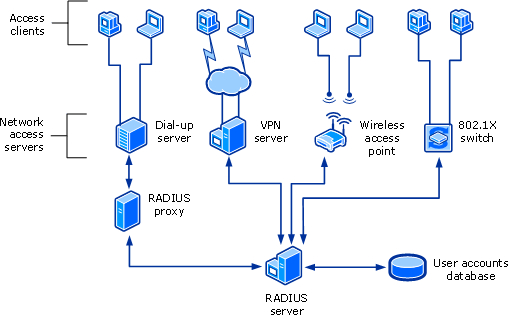
\includegraphics[width=1.0\linewidth]{RADIUS-components}
	\caption {RADIUS Components \cite{RADIUS_components_img}}
	\label{fig:RADIUS_components_img}
	\vspace{-10pt}
\end{figure}
\subsubsection{RADIUS Operation \cite{RADIUS_components}} \label{RADIUS_Operations}
RADIUS messages are sent as UDP messages using the port 1812 for authentication and port 1813 for accounting messages. Some network access servers (NAS) use 1645 and 1646 for authentication and accounting respectively.

A RADIUS data format looks as shown below where the fields are transmitted from left to right.

\begin{lstlisting}
0                   1                   2                   3
0 1 2 3 4 5 6 7 8 9 0 1 2 3 4 5 6 7 8 9 0 1 2 3 4 5 6 7 8 9 0 1
+-+-+-+-+-+-+-+-+-+-+-+-+-+-+-+-+-+-+-+-+-+-+-+-+-+-+-+-+-+-+-+-+
|     Code      |  Identifier   |            Length             |
+-+-+-+-+-+-+-+-+-+-+-+-+-+-+-+-+-+-+-+-+-+-+-+-+-+-+-+-+-+-+-+-+
|                                                               |
|                         Authenticator                         |
|                                                               |
|                                                               |
+-+-+-+-+-+-+-+-+-+-+-+-+-+-+-+-+-+-+-+-+-+-+-+-+-+-+-+-+-+-+-+-+
|  Attributes ...												|
+-+-+-+-+-+-+-+-+-+-+-+-+-+-+-+-+-+-+-+-+-+-+-+-+-+-+-+-+-+-+-+-+

\end{lstlisting}

The code field as shown in the data frame above uses one octet which help identify the type of RADIUS packet.
\begin{itemize}
	\item \textbf{Access-Request:} Sent by the RADIUS client requesting authentication and authorization for a connection.
	\item \textbf{Access-Accept:} It’s the response from the RADIUS server to the client stating that the connection was authenticated and authorized.
	\item \textbf{Access-Reject:} It’s a response from the RADIUS server to the client that the connection attempt failed in authentication.
	\item \textbf{Access-Challenge:} Sometimes the RADIUS server requires more information from the client and sends a challenge as a response the Access-Request message.
	\item \textbf{Accounting-Request:} Sent by the RADIUS client to specify accounting information for an accepted connection.
	\item \textbf{Accounting-Response:} The RADIUS server sends the acknowledgement for the successful receipt and processing of the Accounting-Request message.
	
\end{itemize}

\subsubsection{RADIUS Authentication Mechanism} \label{RADIUS_auth_mechanism}
RADIUS uses the following message codes when communicating between the RADIUS client and server as shown in the figure below.

\begin{figure}[H]
	\centering
	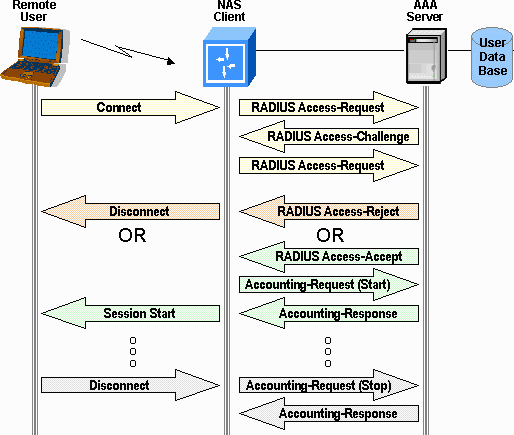
\includegraphics[width=1.0\linewidth]{radius-operation}
	\caption {RADIUS Architecture \cite{Radius_operation_img}}
	\label{fig:RADIUS_architecture}
	\vspace{-10pt}
\end{figure}

\begin{itemize}
	\item \textbf{STEP 1:}When a user makes a connection request, the NAS client sends an Access-Request message to the AAA server, in this case a RADIUS server.
	\item \textbf{STEP 2:}The RADIUS sever responds by sending an Access-Challenge message requesting more information from the user.
	\item \textbf{STEP 3:}The client responds with an Access-Request message with the requested information back to the RADIUS server. The response is typically a username and password information in the form of PPP, PAP or CHAP authentication mechanisms.
	\item \textbf{STEP 4:}The RADIUS server once after validating the received information sends back an Access-Accept information. If not validated, then it sends a Access-Reject message back to the client.
	\item \textbf{STEP 5:}Upon successfully establishing a connection, the client sends an Accounting-Request message to request to start accounting the user.
	\item \textbf{STEP 6:}The RADIUS server responds by sending an Accounting-Response message after successfully starting an accounting session for the connection. Thus, concludes the connection process of the user to the network.
	
\end{itemize}

\subsection{WLAN 802.1x Security \cite{WLAN_802.1x}} \label{802.1x}
Wi-Fi or Wireless Local Area Networks (WLAN’s) have become increasingly more popular in the recent years. The wireless standard IEEE 802.11 has become the most widely adopted standards for wireless broadband internet access. The security considerations however are more complicated in the wireless environment compared to the wired ones. IEEE 802.11 has defined the following two basic security mechanisms for secure access to wireless network.
\begin{itemize}
	\item Entity authentication including shared key and open-system.
	\item Wired Equivalent Privacy (WEP)
\end{itemize}
Both these mechanisms are proven to be severely vulnerable. To enhance the security in wireless networks, 802.11i standard was proposed. This 802.11i standard defines encryption and authentication improvements in addition to introducing protocols for key management and establishment. 802.11i also incorporates the IEEE 802.1x standard as its authentication enhancement. The IEEE 802.1x is a port based network access control used for authenticating and authorizing devices connected by various LAN’s.

The IEEE 802.1x standard is based upon the Extensible Authentication Protocol (EAP), and can use a number of authentication mechanisms which is beyond the scope of the IEEE 802.1x standard. Many authentication mechanisms such as MD5, TLS, TTLS, and PEAP can be used. The IEEE 802.1x uses EAP over LAN (EAPoL) for encapsulating EAP messages between the authenticator and the supplicant. 

There are three main components in the IEEE 802.1x system namely, the supplicant, authenticator and the authentication server. In case of WLAN, the supplicant is usually the mobile device or node, the Access Point (AP) serves as the authenticator and the RADIUS server as the authentication server.  The Port Access Entity (PAE) authenticator relays all the messages between the authentication server and the supplicant. 802.1x is used in this place to enforce the specific authentication mechanism. 

\subsubsection{802.1x Authentication Process} \label{WLAN_802.1x_auth}
Authentication methods of 802.1x include PEAP, MD5 etc. Each method has its own authentication process. The following figure shows the basic EAP based authentication process in Eduroam networks. 

\begin{figure}[H]
	\centering
	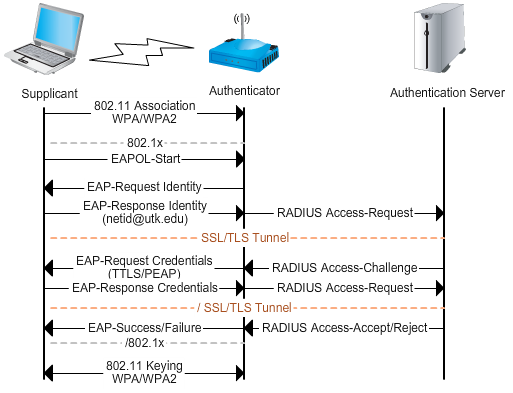
\includegraphics[width=1.0\linewidth]{WLAN_8021x_Auth}
	\caption {IEEE 802.1x WLAN authentication process \cite{WLAN_802.1x_img}}
	\label{fig:WLAN_802.1x_auth_img}
	\vspace{-10pt}
\end{figure}

\begin{itemize}
	\item \textbf{Step 1:} 
	\\ After the association of the supplicant with the authenticator or AP via WPA or WPA2 enterprise, the 802.1x application initiates the EAPOL start message with the authenticator. 
	\item \textbf{Step 2:} 
	\\ The authenticator responds by send a EAP-Request identity message from the supplicant. 
	\item \textbf{Step 3:}
	\\ Once receiving the username as a EAP response from the supplicant, the authenticator then initiates a RADIUS Access-request message with the authentication server. 
	\item \textbf{Step 4:}
	\\ The authenticator receives the RADIUS access challenge from the authentication server and forwards that via a secure SSL/TLS tunnel to the supplicant by encapsulating the EAP-Request credentials message with TTLS/PEAP.
	\item \textbf{Step 5:}
	\\ The supplicant responds with a EAP-Response Credentials message which is typically a username and password to the authenticator via the same secure tunnel, the authenticator forwards the received information as a RADIUS Access-Request message with encapsulation to the authentication server. 
	\item \textbf{Step 6:}
	\\ The authentication server responds with a RADIUS Access-Accept/Reject message to the authenticator. The Authenticator sends this information as a EAP Success/Failure message to the supplicant. 
	\item \textbf{Step 7:}
	\\ The supplicant is now fully associated with the network.
	
\end{itemize}
